
\chapter{ SIFT en GPU}

La correcta paralelización de un algoritmo no es nada trivial. Después de el capitulo anterior, al ver todas las ventajas que tenemos en los GPU`s podríamos decir que son la solución a todo, tristemente no lo son, existen algoritmos que por la estructura del programa y forma de ejecutar el proceso, no se podrían paralelizar. Para saber como analizar si un algoritmo es paralelizable primero debemos dar una definición de que es un programa paralelo:

\begin{center}
\textit{"Programa paralelo es la especificación de dos o mas procesos simultáneos que cooperan entre si con un fin en común"}
\end{center}

Podemos sacar dos aspectos importantes de esta definición el primero es la comunicación, los procesos deben poder compartir información  para poder trabajar simultáneamente sobre un mismo problema; el segundo es la sincronización, es simplemente como organizar a los procesos para que mientras realizan su parte de trabajo sin que se interfieran entre ellos.
Entonces tenemos que cambiar la forma en que programamos, ahora no solo pensaremos como llegar a un objetivo paso a paso, sino  que debemos pensar como muchos procesos trabajaran juntos para alcanzar un objetivo, esto inmediatamente me da la idea de repartir o dividir el trabajo entre todos ellos. 

\pagebreak

Así que para realizar la labor de paralelizar el algoritmo debemos analizar básicamente tres casos de paralelismo:
 
\begin{itemize}
 
	\item \textit{Funcional}: Aquí lo que se divide es el algoritmo, buscamos pasos en el algoritmo que no dependan de otra parte del mismo y los ponemos a ejecutarse simultáneamente en diferentes procesos. Requiere de sincronizan muy cuidadosamente para que las diferentes partes de el algoritmo no interfieran entre si. 
	
	\begin{figure}[h]
			\centering
				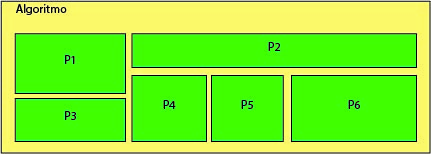
\includegraphics[scale=0.7]{img/funcional.jpg}
			\caption{Todos los procesos son partes diferentes del algoritmo}
	\end{figure}

	\item \textit{Dominio}: Se repartirán los datos en los múltiples procesos los cuales tienen una especificación idéntica. El sincronizan es sencillo en este caso, pero aun así hay que presentar atención ya que podríamos corromper información.
	\begin{figure}[h]
			\centering
				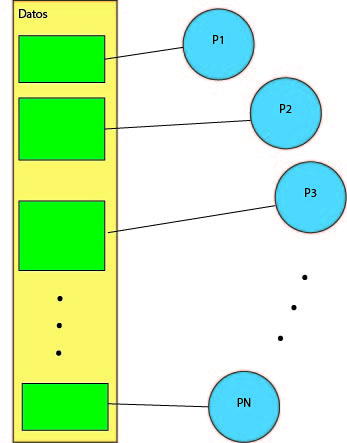
\includegraphics[scale=0.6]{img/dominio.jpg}
			\caption{Todos los procesos tienen la misma especificación }
	\end{figure}

	\item 	\textit{Actividad}: Es una combinación de los dos puntos anteriores.
\end{itemize}

Ahora que tenemos el algoritmo y las herramienta para mejorar su rendimiento por medio de la paraleización. Veremos como analizamos las partes de SIFT para de esta manera adaptarlo al modelo de programación de CUDA.
\pagebreak
\section{Análisis de SIFT para su Paralelización en GPU}

En esta sección se describe como se comunicaran y sincronizar los procesos, así como la estructura que tomara el algoritmo de SIFT, para poder paralelizarlo con CUDA. 

Primero dividiremos en 6 partes el algoritmo de SIFT, como se muestra en la figura 5-3 , estas partes no se ejecutaran simultáneamente, es solo que el algoritmo es bastante largo y al separarlo en estas partes podemos simplificarlo en diferentes kernels, que tendrán una secuencia de ejecución. 


Los kernels de las diferentes partes del algoritmo tienen una estructura en común, básicamente todos tiene como entrada una o mas imágenes, las cuales serán de solo lectura, y obtendremos una imagen o varias de salida. Cada proceso tendrá una sección de la imagen de tamaño  $N \times N$, la cual puede estar traslapada con la de algún otro proceso, pero esta área no requiere de sincronizar entre procesos ya que solo sera para obtener datos, para procesarlos.En la imagen de salida el proceso se le sera asignado solo un pixel de la imagen para escribir, como se puede mostrar en la figura 5-4 las zonas del P1 y P2 están traslapadas y en la imagen de salida, que es como si tuviera un zoom a los pixeles, no escriben en otro que no sea su pixel. 

\pagebreak
Los procesos que se ejecutan sobre la imagen tienen la misma especificación, lo que quiere decir que lo que estamos repartiendo entre los múltiples procesos, serán los datos de entrada, con lo cual estaremos en la categoría de paralelismo de \textit{dominio}.

\begin{figure}[ph]
			\centering
				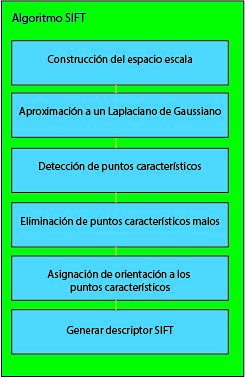
\includegraphics[scale=1]{img/SIFTdiv.jpg}
			\caption{División del algoritmo SIFT a paralelizar}
\end{figure}


\begin{figure}[ph]
			\centering
				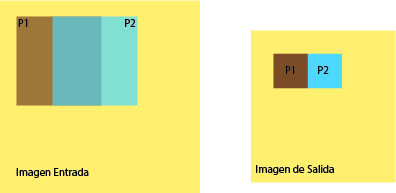
\includegraphics[scale=1]{img/prosImg.jpg}
			\caption{Proceso general de los kenels }
\end{figure}




Cada uno de los kernels serán ejecutados múltiples veces, este trabajo sera desempeñado por el anfitrión (CPU) de forma secuencial, esto es importante ya que cada uno de estos kernels es lanzado sin importar que el anterior acabara de ejecutarse, si múltiples kernels son lanzados y tiene la misma especificación pero trabajan con diferentes secciones de los datos no existe problema. Pero si el anfitrión llegara a lanzar un kernel que tiene una especificación diferente a la de un banco de kernels iguales lanzados anteriormente y estos no han finalizado puede existir riesgo de corromper los datos. Entonces debemos de sincronizar , como se puede ver en la figura 5-5, al  dispositivo (GPU) con el anfitrión (CPU) para evitar caer en este tipo de errores.

\begin{figure}[ph]
			\centering
				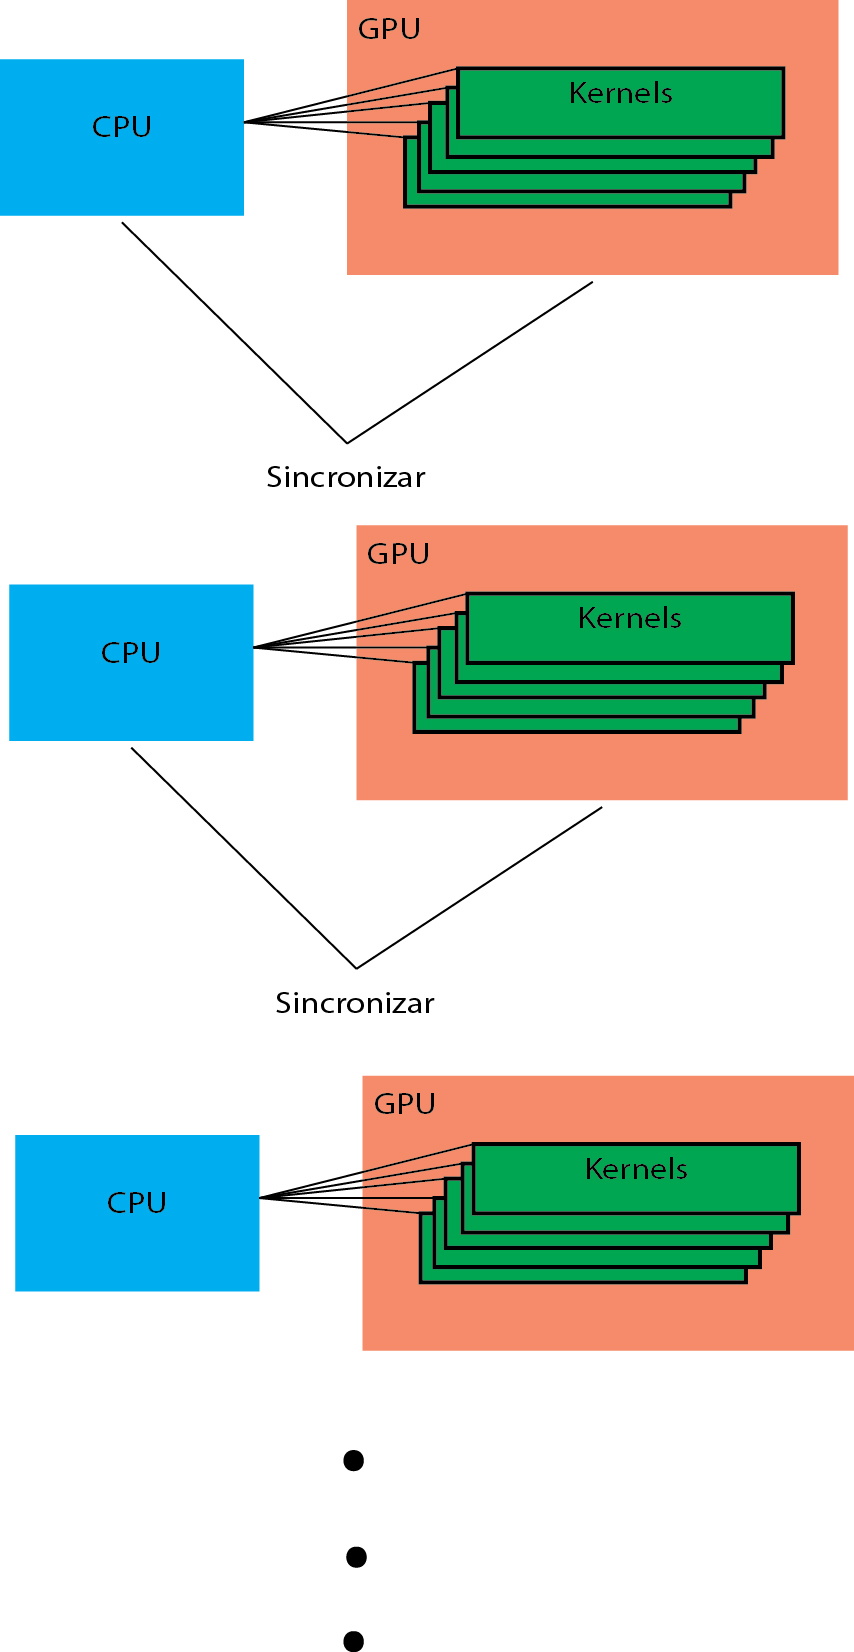
\includegraphics[scale=1]{img/lanzamiento.jpg}
			\caption{Lanzamiento de Kernels }
\end{figure}


\pagebreak
\section{Implementación}

Ahora que conocemos la estructura general de la solución, plantearé como construí cada una de las partes en las que dividí el algoritmo de SIFT, figura 5-3,  para poder adaptarlo a el modelo de programación de CUDA.

\subsection{Construcción del espacio escala y aproximación a un Laplaciano de Gaussiano}

Recordando un poco, el espacio escala se forma a partir de suavizar la imagen original a diferentes niveles de detalles, lo que hice fue cambiar el filtro gaussiano por uno que se aproximara a el Laplaciano de Gaussiana, que seria una diferencia de Gausianas. 

$$D(x,y;\sigma) = (G(x,y;k\sigma) - G(x,y;\sigma)) * I(x,y)$$ 

Para ello obtendremos los filtros Gaussianos con la ayuda de la librería OpenCV, y los restamos para así obtener los filtros que aplicaremos en cada octava. Quedando como los de las figura 5-6.


\begin{figure}[h]
			\centering
				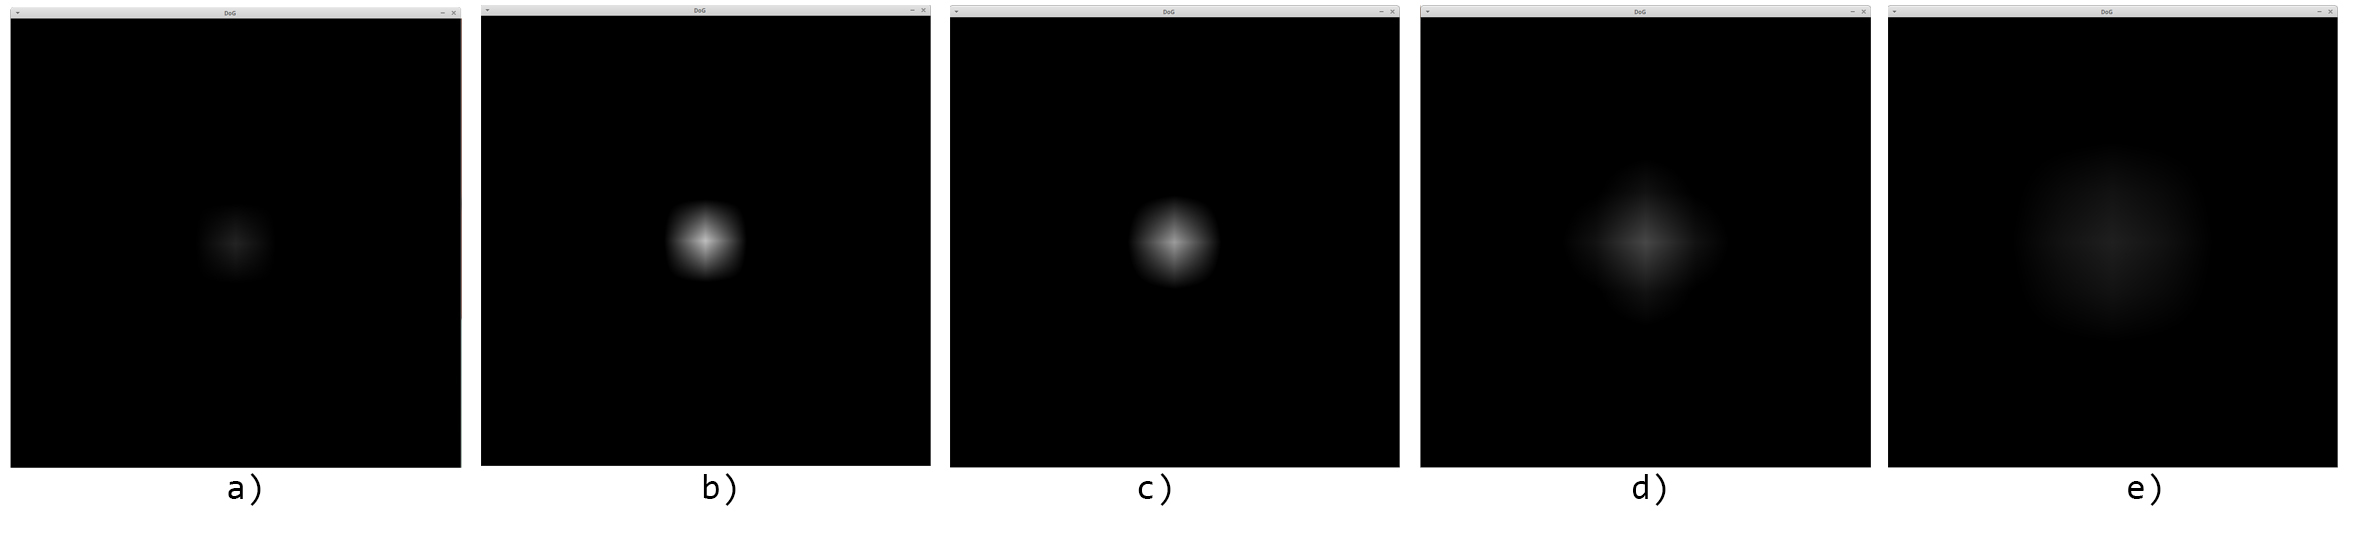
\includegraphics[scale=0.2]{img/DoG.jpg}
			\caption{Filtros}
\end{figure}



 


También usaré OpenCV para cambiar el tamaño de las imágenes, para cada octava.

La sección de esta parte, de las que dividí el algoritmo, que es altamente paralelizable es al momento de hacer la convolución. Por este motivo lo que hice fue desarrollar un kernel, se puede encontrar en el apéndice A, que realice la convolución de una imagen y un filtro.

\pagebreak
 
La idea es que estos kernels son lanzados por el anfitrión, se lanzaran tantos kernels como imágenes se necesitan para crear el espacio escala. Los kernels sera ejecutados de forma concurrente. 

La funcionalidad del kernel es, para cada pixel en la imagen de salida se asigna un hilo de diferentes bloques, y estos se encargaran con los datos de entrada, la imagen y el filtro, implementar la operación de convolución.\\

\begin{algorithm}[H]
\caption{Calculo de la convolución para cada imagen del espacio escala}
 \KwData{ImgEntrada, Filtro}
 \KwResult{Img }
 Para cada pixel en ImgEntrada asigna un hilo\;
 
 \ForAll{hilos}
 {
	\eIf{Img.pixel es orilla}
	{
		Img.pixel=0;
	}{
		
		Img.pixel= ImgEntrada.zona * Filtro; 
		\\
		\tcp{Donde * es el operador para la convolución}			
		}
 }
	

\end{algorithm}
\begin{figure}[ph]
			\centering
				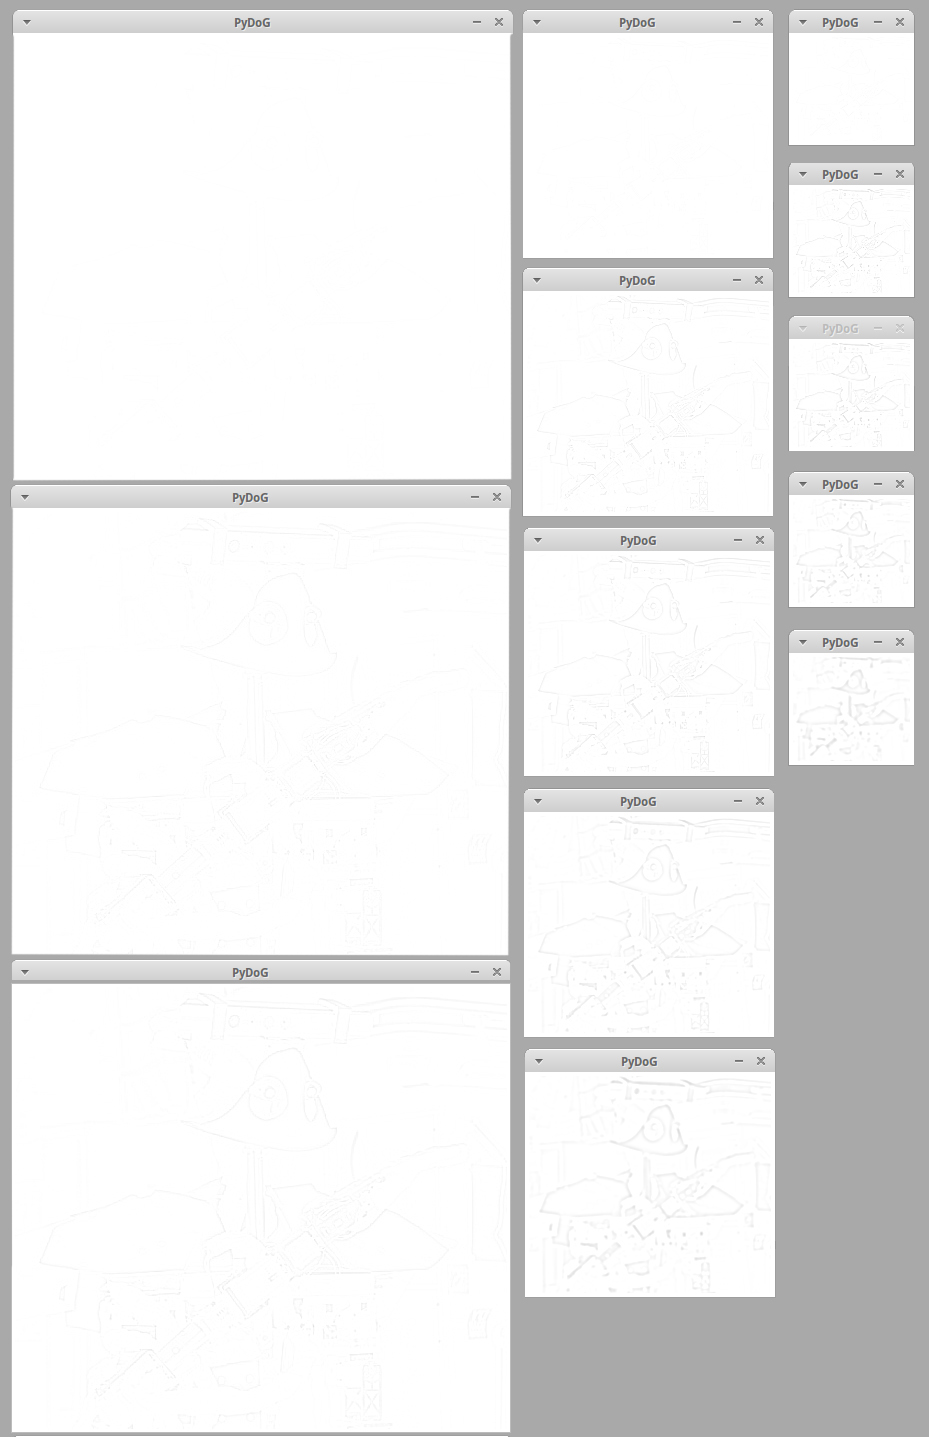
\includegraphics[scale=0.45]{img/pyDoGT.jpg}
			\caption{Espacio Escala de Diferencia de Gaussianas}
\end{figure}


El resultado es como el de la figura 5-7, tendremos imágenes muy similares para cada una de las octavas. 
\\\\\\\\\\\\\\\\\\\\


\subsection{Detección de puntos característicos}
En el espacio escala, obtenido anteriormente, buscaré los puntos extremos. A lo que nos referimos con esto es que en $D(x,y,\sigma)$ buscaré las ubicaciones máximas y mínimas, cada punto es comparado con sus ocho vecinos en la misma imagen y con sus otros dieciocho vecinos de escala, nueve en la imagen de arriba y nueve en la imagen de abajo. Solo se selecciona la ubicación si el pixel tiene un valor mayor o menor a todos sus vecinos.\\


\begin{algorithm}[H]
\caption{Búsqueda de puntos extremos}
 \KwData{ImgArriba, Img , ImgAbajo }
 \KwResult{ImgMascara}
 Para cada pixel en Img asigna un hilo\;
 
 \ForAll{hilos}
 {
	\eIf{Img.pixel es orilla}
	{
		ImgMascara.pixel=0\;
	}{
		\ForAll{pixel vecino a Img en ImgArriba, ImgAbajo e Img }
		{
			Compara cada pixel vecino con el pixel asignado al hilo\;
			\eIf{si todos los vecinos son menores o mayores}
			{
				ImgMascara.pixel = 1\;			
			}{
				ImgMascara.pixel = 0\;
			
			}
		
		}
		
	}
 }
	
\end{algorithm}


Como podemos ver en el algoritmo 2, lo que hacemos en el kernel es a cada hilo se le va a asignar un pixel de la imagen de entrada \texttt{Img} para compararla con sus vecinos y asi poder determinar si es un punto extremo.\\ \pagebreak
 
\begin{figure}[h]
			\centering
				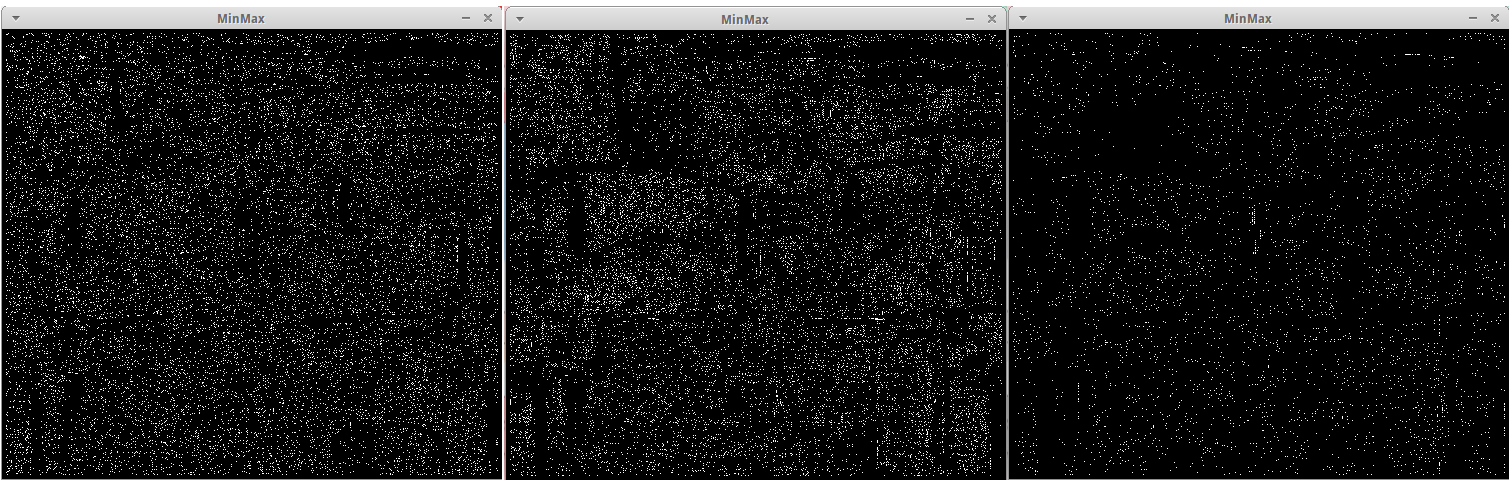
\includegraphics[scale=0.3]{img/minmaxs.jpg}
			\caption{Mascara}
\end{figure} 
 
La imagen de salida terminara siendo una mascara binaria si existe un punto extremo, pondrá un pixel en blanco y donde no lo dejara en negro, como se muestra en la figura 5-8; Podemos encontrar la implementación de este algoritmo en el apéndice B.\\\\\\\\\\\\\\\\\\\\\\\\\\\\\\\\\\\\\\\ \pagebreak






\subsection{Eliminación de puntos característicos malos}

Ahora filtraré los puntos extremos que encontramos anteriormente. Existen dos casos donde los puntos extremos anteriormente seleccionados tendrían que ser eliminados:
	\begin{enumerate}
		\item El punto tiene un contraste muy bajo.
		\item El punto está localizado sobre un borde.
	\end{enumerate}		

\begin{algorithm}[H]
\caption{Eliminación de puntos característicos malos}
 \KwData{Img , ImgMascara}
 \KwResult{ImgMascara}
 Para cada pixel en Img asigna un hilo\;
 
 \ForAll{hilos}
 {
	\If{ImgMascara.pixel es mayor que 0}
	{
		\If{Img.pixel tiene contraste bajo o esta en un borde}
		{
			ImgMascara.pixel=0;
		}
	
				
	}
	
	
		
}
	
\end{algorithm}

Obtendremos una mascara muy parecida a la de la figura 5-9 pero esta vez tendremos muchos menos pixeles en color blanco. En el apéndice C podemos ver mas detalladamente como es que se realizo la implementación de esta parte de el algoritmo de SIFT.

\begin{figure}[h]
			\centering
				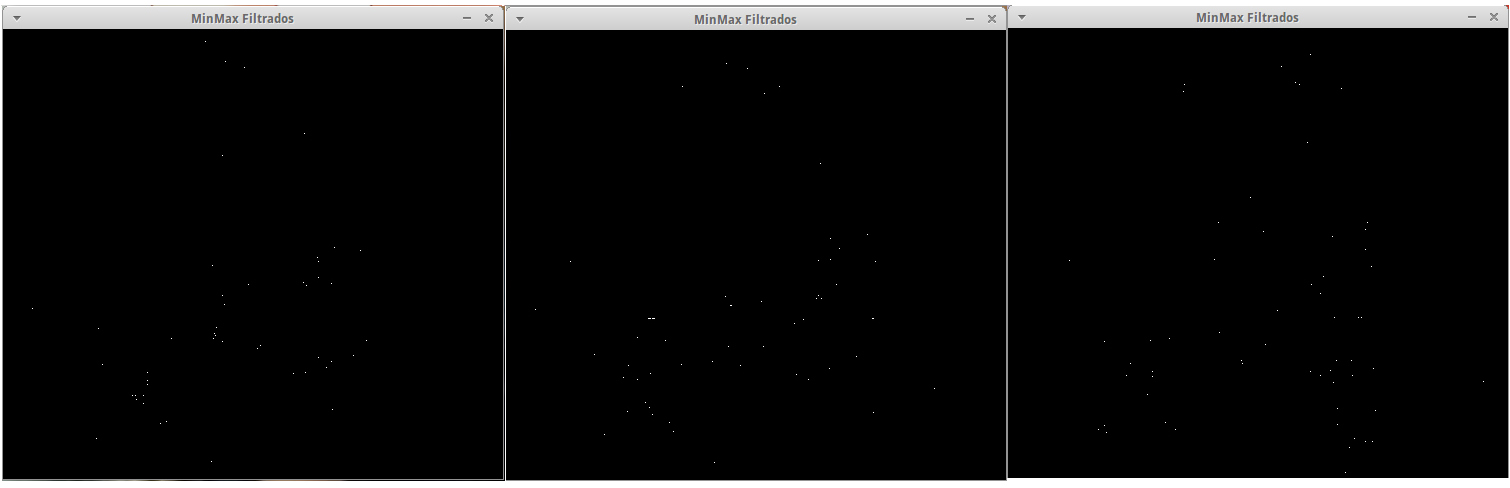
\includegraphics[scale=0.3]{img/minmax.jpg}
			\caption{Mascara Filtrada}
\end{figure}



\subsection{Asignación de orientación a los puntos característicos}

Encontrar la orientación de cada punto característico, basado en propiedades locales de la imagen, es importante para que el descriptor sea invariante a la rotación.


\begin{algorithm}[H]
\caption{Eliminación de puntos característicos malos}
 \KwData{Img}
 \KwResult{ImgMagnitud, ImgOrientacion}
 Para cada pixel en Img asigna un hilo\;
 
 \ForAll{hilos}
 {
	Calcular magnitud en Img.pixel\;
	Calcular orientación en Img.pixel\;
	
	ImgMagnitud.pixel= magnitud\;
	ImgOrientacion.pixel=orientación\;
	
}
\end{algorithm}



Para esta parte lo mejor fue dividir en dos kernels este proceso uno para calcular las magnitudes y orientaciones de los gradientes. En el apéndice D se encuentra la implementación de este kernel.

$$m(x,y) = \sqrt{ (L(x+1,y)-L(x-1,y))^2 + (L(x,y+1)-L(x,y-1))^2 }$$		
$$\theta(x,y) =  \tan^{-1} \left(\frac{L(x,y+1)-L(x,y-1)}{L(x+1,y)-L(x-1,y)}\right)$$


Y la otra sera donde tendremos que obtener los histogramas para cada punto característico y asignar una orientación dominante. En el apéndice E, encontraremos su implementación. 

\pagebreak

\begin{algorithm}[H]
\caption{Eliminación de puntos característicos malos}
 \KwData{Img , ImgMascara, ImgMagnitud, ImgOrientacion}
 \KwResult{PuntosCaracteristicos}
 Para cada pixel en Img asigna un hilo\;
 
 \ForAll{hilos}
 {
	\If{ImgMascara.pixel es mayor que 0}
	{
		Realizar el histograma de a zona al rededor de el punto característico\;
		Encontrar cuales son los valores mas altos más altos\;
		Encontrar una orientación dominante con los puntos mas altos\;
		Almacenar la orientación y la ubicación de ese punto característico\; 
				
	}
}
	
\end{algorithm}




\begin{figure}[h]
			\centering
				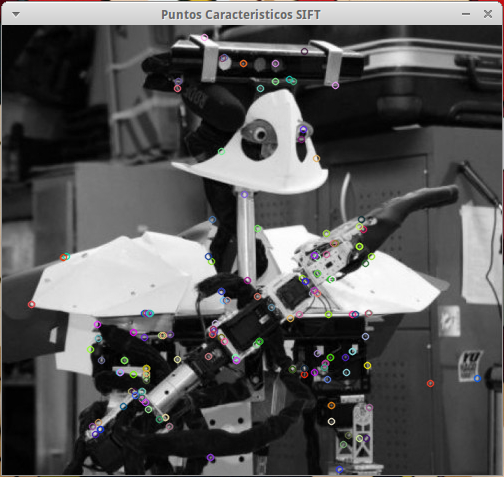
\includegraphics[scale=1]{img/KeyPoints.png}
			\caption{Puntos característicos }
\end{figure}



























%%\subsection{Generar Descriptor SIFT}
